%! Author = zkyoto
%! Date = 10.01.2024

\LARGE
\textbf{Linux: стандартные средства для наблюдения счетчиков ядра.}\\
\normalsize

Историческая утилита - sar (system activity reporter). Существует почти с самого начала Linux, имеет самый обширный сбор счётчиков. \\
Собирает статистику по:
\begin{itemize}
    \item пейджингу (-В)
    \item свопингу (-W)
    \item вводу-выводу (-b,-d)
    \item смонтированным системам (-F)
    \item прерываниям (-I)
    \item управлению питанием (-m)
    \item сети (-n)
    \item процессорам (-Р,-u)
    \item очереди процессов и загрузке (-q,-w)
    \item памяти (-r)
    \item области подкачки (-s)
    \item терминалам (-у)
\end{itemize}
Важная особенность: на утилиту можно настроить кронячку - запуск по расписанию со сбором информации и сохранением логов,
которые потом читаем. Другие утилиты так настраивать нельзя.\\

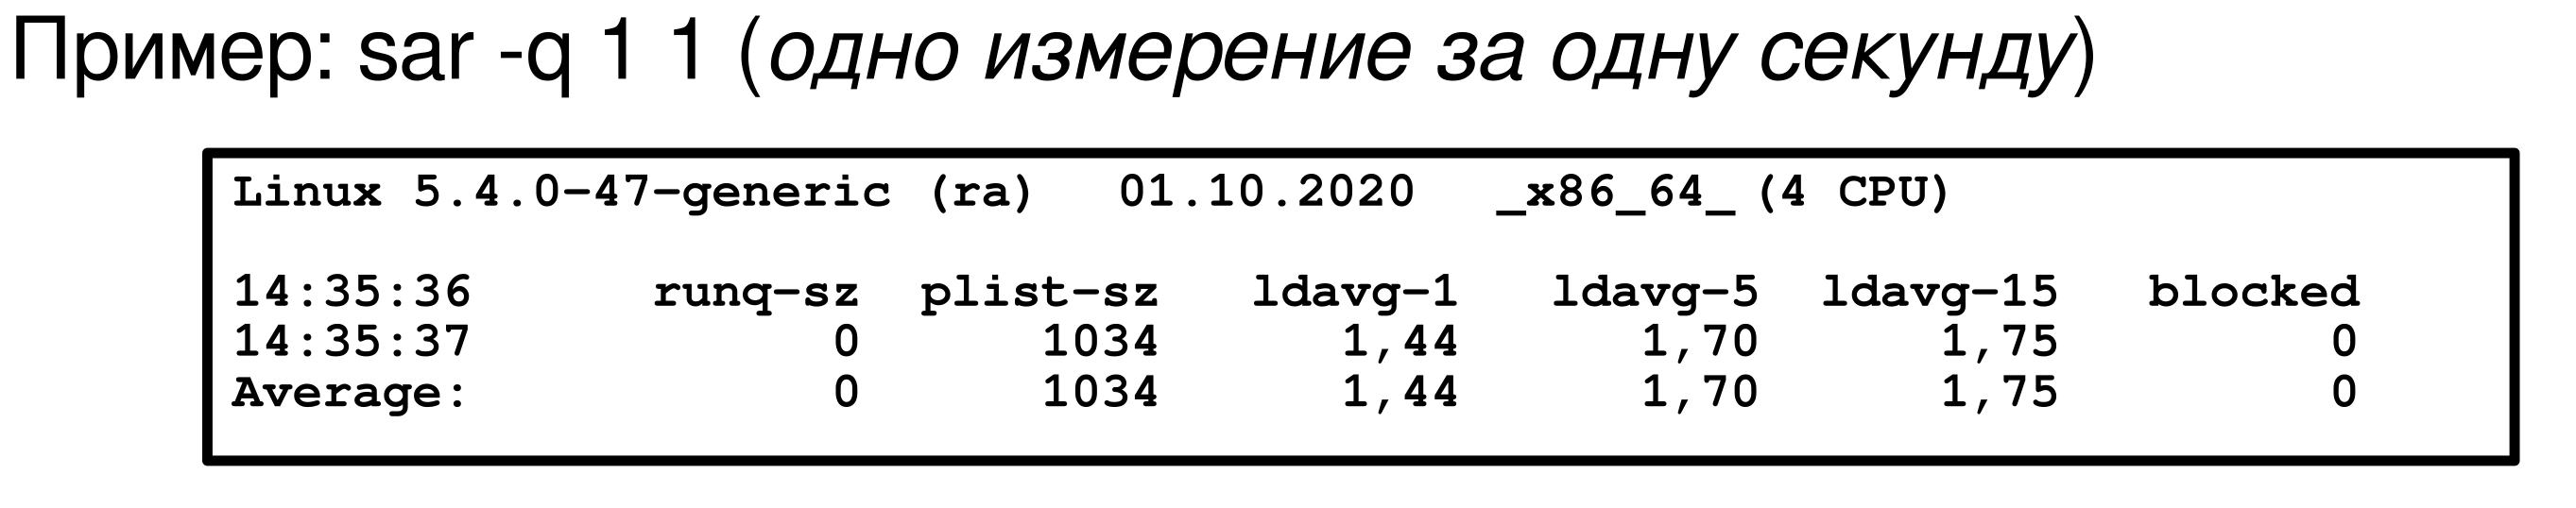
\includegraphics[width = 400]{/Users/zkyoto/workspace/OS_exam/tickets/img/70.1}
\newpage